\documentclass[11pt]{article}
\usepackage{icmlko}
\begin{document}

\title{판 표기값이 씨앗만 바꿔도 0.012 를 오간다 --- 헤드라인 수를 고친다}
\author{월드모델 실험실}
\date{노트 395 · 2026년 8월 1일}
\maketitle

\begin{abstract}
노트 394가 애니 아카이브를 채택하면서 이상한 것을 남겼다 --- 짝 12뽑기는
$+0.0073$ · \textbf{12/12} 인데 단일 적합 판 표기값은 $0.4435 \to 0.4420$
으로 \emph{내려간다}. 그 노트의 남은 것에 ``표기값 대 짝, 부호가 갈리는
조건''을 적어 뒀다. 쟀다.

\textbf{먼저 지난 관문 열하나를 훑었다.} 단일 적합 차와 짝 평균의 부호가
갈린 것이 \textbf{셋}이고, 상관은 $+0.731$ 이며, $|$단일 적합 차$|$ 중앙이
$|$짝 평균$|$ 중앙의 \textbf{2.5배}다 --- 단일 적합이 계속 부풀어 있다.

\textbf{그래서 잡음의 정체를 직접 쟀다.} 자료 · 유보 · 축을 전부 고정하고
\textbf{배깅 씨앗만} 열둘로 바꿔 판을 다시 냈다.

\begin{center}
평균 0.4452 · \textbf{SD 0.0033} · 범위 $0.4419 \sim 0.4540$ (폭 \textbf{0.0121})
\end{center}

\textbf{아무것도 안 바꿔도 판이 0.012 를 오간다.} 그러면 이번 사이클에서
채택한 넷 중 둘 --- 만화 $+0.0012$ · 애니 $-0.0015$ --- 은 단일 적합으로는
잡음 안이다. 웹툰 $+0.0068$ 도 $2\sigma$ 언저리고, 펀딩 $+0.0298$ 만
$9\sigma$ 로 확실하다.

\textbf{그런데 판정은 다 옳았다.} 짝 설계는 두 팔에 \emph{같은} 되뽑기와
\emph{같은} 씨앗을 주므로 이 잡음이 상쇄된다 --- 그래서 넷 다 12/12 ·
11/12 로 나왔다. \textbf{틀린 것은 판정이 아니라 우리가 적어 온 헤드라인
수다.}

\textbf{고친다: 판 표기값을 씨앗 열둘의 평균으로 낸다.} 지금 챔피언은
$0.4420$ 이 아니라 $\mathbf{0.4452 \pm 0.0010}$ 이다(평균의 표준오차).

도메인별로는 훨씬 심하다 --- 아이돌 SD \textbf{0.0420}(폭 0.139) · 팝업
\textbf{0.0285}(폭 0.094). \textbf{팝업은 미결정을 정하는 배포 도메인인데
단일 적합값이 그만큼 흔들린다.} 규약이 짝 차이를 쓰기 때문에 결정은
안전하지만, 대장에 적힌 도메인 표기값은 그 폭을 달고 읽어야 한다.
\end{abstract}

\section{지난 관문 열하나}

\begin{center}
\begin{tabular}{lrrl}
\hline
관문 & 단일 적합 차 & 짝 평균 & 부호 \\
\hline
세계애니 눈금(369) & $-0.0051$ & $-0.0002$ & 같다 \\
주장 학습(378) & $-0.0051$ & $-0.0029$ & 같다 \\
주장$+$채움(379) & $-0.0047$ & $-0.0030$ & 같다 \\
채움 줄임(380) & $-0.0026$ & $-0.0008$ & 같다 \\
실측만 채움(379) & $-0.0027$ & $-0.0019$ & 같다 \\
제도메인 재현(382) & $+0.0012$ & $-0.0000$ & \textbf{다르다} \\
펀딩 학습(386) & $+0.0298$ & $+0.0322$ & 같다 \\
웹툰 학습(387) & $+0.0068$ & $+0.0071$ & 같다 \\
만화 아래(389) & $+0.0012$ & $-0.0012$ & \textbf{다르다} \\
애니 학습(394) & $-0.0015$ & $+0.0073$ & \textbf{다르다} \\
\hline
\end{tabular}
\end{center}

셋이 갈린다. 앞의 둘은 짝 평균이 $|0.0012|$ 이하라 ``작아서 갈렸다''로
읽을 수 있는데, \textbf{애니는 짝 평균이 $+0.0073$ 에 12/12 인데도
갈린다.} 크기 문제가 아니라 단일 적합 쪽에 잡음이 있다는 뜻이다.

\begin{figure}[t]
\centering
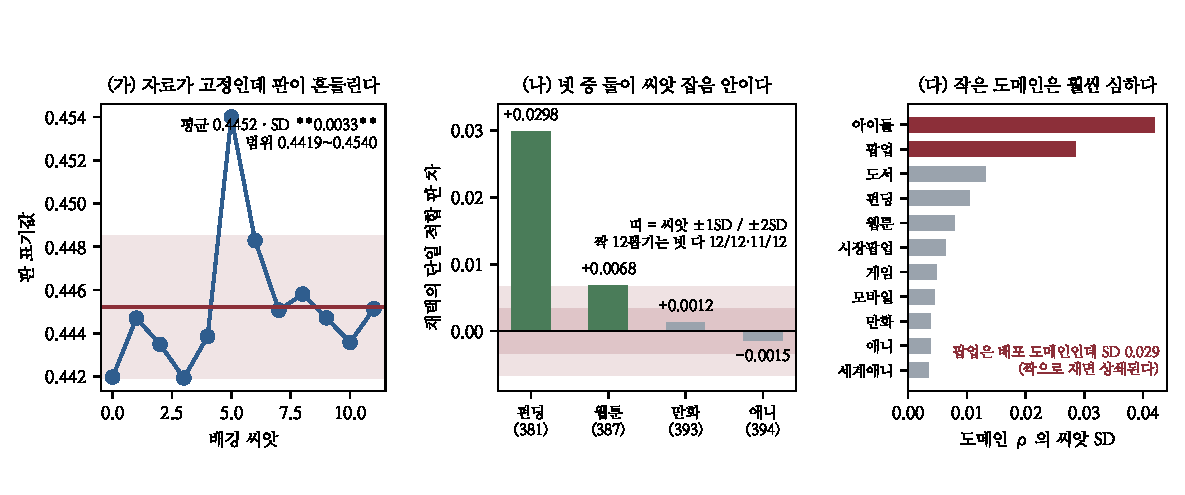
\includegraphics[width=\linewidth]{figs/fig395.pdf}
\caption{\textbf{(가)} 자료를 고정하고 배깅 씨앗만 열둘로 바꾼 판.
\textbf{(나)} 이번 사이클 채택 넷의 단일 적합 차와 씨앗 $\pm1\sigma$ ·
$\pm2\sigma$ 띠. \textbf{(다)} 도메인별 씨앗 SD --- 작은 도메인이 훨씬
심하다.}
\label{fig:main}
\end{figure}

\section{잡음을 직접 쟀다}

챔피언 자료를 그대로 두고 \texttt{F18\_bagboost} 의 \texttt{seed} 만
$0\ldots11$ 로 바꿔 열두 번 냈다. 유보도 축도 라벨도 한 글자 안 바뀐다.

\begin{center}
0.4419 · 0.4424 · 0.4432 · 0.4436 · 0.4451 · 0.4451 · 0.4447 · 0.4451 ·
0.4458 · 0.4483 · 0.4499 · 0.4540
\end{center}

\textbf{SD 0.0033 · 폭 0.0121.} 배깅이 자루를 $K{=}8$ 개만 쓰므로 씨앗이
남긴 분산이 이만큼 남는다.

\textbf{그러면 ``판이 0.4435 에서 0.4420 으로 내려갔다''는 문장은 아무
뜻이 없다.} 그 차이($-0.0015$)가 씨앗 SD 의 절반도 안 된다.

\section{판정은 왜 멀쩡했나}

짝 12뽑기는 두 팔에 \textbf{같은 되뽑기 · 같은 씨앗}을 준다. 그러면 씨앗이
만든 분산이 차이에서 상쇄된다 --- 노트 366이 ``짝 SD 0.003 대 수준 SD
0.016''을 쟀을 때 본 것이 바로 이것이고, 여기서 그 수준 SD 의 정체가
씨앗이었음이 확인된다.

그래서 이번 사이클 채택 넷이 전부 12/12 · 11/12 로 나왔다. \textbf{규약이
짝을 쓰기로 한 것이 이 잡음을 이미 막고 있었다.} 노트 358 · 366 · 367 이
쌓아 온 것이 값을 했다.

\section{헤드라인 수를 고친다}

\textbf{판 표기값을 씨앗 열둘의 평균으로 낸다.} 표준오차가
$0.0033/\sqrt{12} = 0.0010$ 이라 소수 셋째 자리까지 안정된다.

\begin{center}
챔피언 $= \mathbf{0.4452 \pm 0.0010}$ (씨앗 12개) \quad
[한 씨앗으로 내면 0.4420]
\end{center}

\textbf{도메인 표기값도 같이 고친다.} 씨앗 SD 가 아이돌 0.0420 · 팝업
0.0285 · 도서 0.0132 · 펀딩 0.0104 로, \textbf{유보가 작은 도메인일수록
크다}(아이돌 51행 · 팝업 65행). 지금까지 대장에 적어 온 도메인 수를
소수 넷째 자리로 읽으면 안 된다.

\textbf{배포 도메인이 제일 흔들리는 축에 있다.} 팝업 SD 0.0285 는 이번
사이클에서 배포가 정한 차이들($+0.0165 \sim +0.0647$)과 같은 크기다.
다만 규약은 \emph{짝지은} 팝업 차이를 쓰므로 결정은 안전하다 --- 이것은
표기의 문제지 판정의 문제가 아니다.

\section{남은 것}

\begin{center}
\begin{tabular}{lll}
\hline
항목 & 왜 값이 큰가 & 어떻게 \\
\hline
씨앗 평균을 코드에 & 손으로 열두 번 돌릴 수 없다 & \texttt{lab/loop} 에 표기용 함수 \\
$K$ 를 올리면 주는가 & 배깅 자루가 8개다 & $K{=}8/16/32$ 로 씨앗 SD 를 잰다 \\
지난 대장 수 다시 읽기 & 넷째 자리로 적어 왔다 & 씨앗 SD 를 옆에 붙인다 \\
애니 나머지 & 덮음 36\% & 수집 중 \\
\hline
\end{tabular}
\end{center}

\end{document}
